\documentclass[oneside]{amsart}

\usepackage[utf8]{inputenc}
\usepackage{amsthm,mathtools,stmaryrd,amssymb,graphicx}
\usepackage{booktabs}
\usepackage[all]{xy}
\usepackage[protrusion=true,expansion=true]{microtype}
\usepackage{xspace}

\usepackage[natbib=true,style=numeric,maxnames=10]{biblatex}
\usepackage[babel]{csquotes}
\bibliography{paper-filmat.bib}

\graphicspath{{images/}}

\usepackage{pifont}
\newcommand{\cmark}{\ding{51}}
\newcommand{\xmark}{\ding{55}}

\title[]{Exploring mathematical objects from custom-tailored mathematical universes}
\author{Ingo Blechschmidt}
\address{Università di Verona \\
Department of Computer Science \\
Strada le Grazie 15 \\
37134 Verona, Italy}
\email{iblech@speicherleck.de}

\theoremstyle{definition}
\newtheorem{defn}{Definition}[section]
\newtheorem{ex}[defn]{Example}

\theoremstyle{plain}
\newtheorem{prop}[defn]{Proposition}
\newtheorem{cor}[defn]{Corollary}
\newtheorem{lemma}[defn]{Lemma}
\newtheorem{thm}[defn]{Theorem}
\newtheorem{scholium}[defn]{Scholium}

\theoremstyle{remark}
\newtheorem{rem}[defn]{Remark}
\newtheorem{question}[defn]{Question}
\newtheorem{speculation}[defn]{Speculation}
\newtheorem{caveat}[defn]{Caveat}
\newtheorem{conjecture}[defn]{Conjecture}

\newcommand{\xra}[1]{\xrightarrow{#1}}
\newcommand{\XXX}[1]{\textbf{XXX: #1}}
\newcommand{\aaa}{\mathfrak{a}}
\newcommand{\bbb}{\mathfrak{b}}
\newcommand{\mmm}{\mathfrak{m}}
\newcommand{\I}{\mathcal{I}}
\newcommand{\J}{\mathcal{J}}
\newcommand{\E}{\mathcal{E}}
\newcommand{\F}{\mathcal{F}}
\newcommand{\B}{\mathcal{B}}
\newcommand{\NN}{\mathbb{N}}
\newcommand{\RR}{\mathbb{R}}
\newcommand{\ZZ}{\mathbb{Z}}
\renewcommand{\P}{\mathcal{P}}
\renewcommand{\O}{\mathcal{O}}
\newcommand{\defeq}{\vcentcolon=}
\newcommand{\op}{\mathrm{op}}
\DeclareMathOperator{\Spec}{Spec}
\DeclareMathOperator{\Hom}{Hom}
\DeclareMathOperator{\Mod}{Mod}
\DeclareMathOperator{\Sh}{Sh}
\DeclareMathOperator{\PSh}{PSh}
\newcommand{\Set}{\mathrm{Set}}
\newcommand{\Eff}{\mathrm{Ef{}f}}
\renewcommand{\_}{\mathpunct{.}\,}
\newcommand{\effective}{ef{}fective\xspace}
\newcommand{\?}{\,{:}\,}
\newcommand{\realizes}{\Vdash}
\newcommand{\notnot}{\emph{not~not}\xspace}

\newcommand{\stacksproject}[1]{\cite[{\href{https://stacks.math.columbia.edu/tag/#1}{Tag~#1}}]{stacks-project}}

\renewcommand{\paragraph}[1]{\noindent\textbf{#1.}}

\begin{document}

\begin{abstract}
  foo
\end{abstract}

\maketitle
\thispagestyle{empty}

\noindent


\section{Unsorted}

Toposes can be pictured as ``universes in which we can do mathematics in'' in
much the same way as models of set theory can be viewed in this way. In fact,
to any model~$M$ of a set theory such as~$\mathbf{ZF}$ or~$\mathbf{ZFC}$, there
is a topos~$\Set_M$ such that a statement holds in the internal language
of~$\Set_M$ if and only if it holds in~$M$.\footnote{The topos~$\Set_M$ can be
described as follows: Its objects are the elements of~$M$, that is the things
which~$M$ believes to be sets, and its morphisms are those things which~$M$
believes to be maps. The topos~$\Set_M$ validates the axioms of
$\mathbf{ETCS}$~\cite{XXX}, and for models which are not elementarily
equivalent, their associated toposes will not be equivalent.} This
includes~$V$, the trivial inner model consisting of all sets there are, in case
such a thing exists in one's chosen ontology; in this case the associated
topos~$\Set_V$ is the category of all sets, and a statement holds in~$\Set_V$
if and only if it's true in the ordinary mathematical sense.

Carrying the analogy further, just as using forcing and other techniques we can
construct new models of set theory from given ones, thereby exploring the
set-theoretic multiverse, we can construct new toposes from given toposes.
However, there are two important differences between the notion of mathematical
universe as provided by toposes and as provided by models of set theory, both
regarding the subject matter and the reasons for why we are interested in them.

Firstly, toposes are more general than models of set theory. By definition, a
model of~$\mathbf{ZFC}$ will always satisfy the axioms of~$\mathbf{ZFC}$; in
contrast, most toposes do not even validate the law of excluded middle, much
less so the axiom of choice (which implies the law of excluded middle in
presence of the remaining axioms of intuitionistic Zermelo--Fraenkel set
theory~\cite{XXX}). This failure of classicality is often for interesting
geometric or algebraic reasons instead of because of logical issues, as will be
detailed in Section~\ref{several-toposes}.

Secondly, there is a difference in motivation. The main philosophical reason
for studying models of set theory is to study which notions of sets are
coherent: Does the cardinality of the reals need to be the cardinal directly
succeeding~$\aleph_0$, the cardinality of the naturals? No, there are models of
set theory in which the continuum hypothesis fails. Do non-measurable sets of
reals need to exist? No, in models of~$\mathbf{ZF}+\mathbf{AD}$,
Zermelo--Fraenkel set theory plus the axiom of determinacy, it's a theorem that
every subset of~$\RR^n$ is Lebesgue-measurable. Can the axiom of choice be
added to the axioms of~$\mathbf{ZF}$ without causing inconsistency? Yes, if~$M$
is a model of~$\mathbf{ZF}$ then~$L^M$, the set of definable sets of~$M$, is a
model of~$\mathbf{ZFC}$.~\cite{XXX, maybe SEP?}

While toposes can be used for similar such purposes, and indeed have been,
especially to explore the various intuitionistic notions of sets, an important
aspect of topos theory is that toposes are used to explore the standard
mathematical universe: Truth in the \effective topos tells us what is
computable; truth in sheaf toposes tells us what's true locally, in a fashion
which depends continuously on parameters; the little Zariski topos of a general
commutative ring can be used to pretend that the given ring is a field; toposes
adapted to synthetic differential geometry can be used to rigorously work with
infinitesimals. All of these examples will be presented in more detail in
Section~\ref{several-toposes}.

In a certain precise way, toposes allow us to study the common objects of
mathematics from a different point of view -- one such view for every topos --
and it is a beautiful and intriguing fact that with the sole exception of the
law of excluded middle, the laws of logic apply to mathematical objects also
when viewed through the lens of a specific topos.


\section{Exploring the \effective topos}

% XXX introduction
% XXX mention connection to realizability

\begin{tabular}{lll}
  \toprule
  Statement & in $\Set$ & in $\Eff$ \\
  \midrule
  Any natural number is prime or not prime. & \cmark{} (trivially so) & \cmark \\
  There are infinitely many primes. & \cmark & \cmark \\
  Any function $\NN \to \NN$ is the zero function or not. & \cmark{} (trivially so) & \xmark \\
  Any function $\NN \to \NN$ is computable by a Turing machine. & \xmark & \cmark{} (trivially so) \\
  Any function $\RR \to \RR$ is continuous. & \xmark & \cmark \\
  \bottomrule
\end{tabular}

\subsection{``Any natural number is prime or not.''} Even without knowing what
a prime number is, one can safely judge this statement to be true in
the standard topos, since it is just an instance of the law of excluded middle.

By the Kripke--Joyal semantics, saying that it's true in the \effective topos
amounts to saying that there is a Turing machine which, given a natural
number~$n$ as input, terminates with a correct judgment whether~$n$ is prime or
not. Such a Turing machine indeed exists -- writing such a program is often a
first exercise in programming courses. Hence the statement is also true in the
\effective topos, but for the nontrivial reason that such a machine exists.


\subsection{``There are infinitely many primes.''} A first-order formalization
of this statement is ``for any natural number~$n$, there is a natural
number~$p$ which is greater than~$n$'', and is known to be true in the standard
topos by any of the many proofs of this fact.

Its external meaning when interpreted in the \effective topos is that there exists
a Turing machine which, given a natural number~$n$ as input, terminates with a
prime number~$p > n$ as output. Such a Turing machine exists, hence the
statement is true in the \effective topos.


\subsection{``Any function~$\NN \to \NN$ is the zero function or not.''} More
formally, the statement is
\[ \forall f \? \NN^\NN\_
  \bigl((\forall n \? \NN\_ f(n) = 0) \vee
  \neg
  (\forall n \? \NN\_ f(n) = 0)\bigr). \]
By the law of excluded middle, this statement is trivially true in the standard
topos.

Its meaning when interpreted in the \effective topos is that there exists a
Turing machine~$M$ which, given the description of a Turing machine~$F$ which
computes a function~$f : \NN \to \NN$ as input, terminates with a correct
judgment of whether~$f$ is the zero function or not. Such a machine~$M$ does
not exist, hence the statement is false in the \effective topos.

A formal proof that such a machine~$M$ does not exist will reduce its assumed
existence to the undecidability of the halting problem. Intuitively, the issue
is the following. Turing machines are able to simulate other Turing machines.
Hence~$M$ could simulate~$F$ on various inputs to search the list of
function values~$f(0), f(1), \ldots$ for a nonzero number. In case that after
a certain number of steps a nonzero function value is found, the machine~$M$
can correctly output the judgment that~$f$ is not the zero function. But if the
search only turned up zero values, it cannot come to any verdict -- it cannot
rule out that a nonzero function value will show up in the as yet unexplored
part of the function.


\subsection{``Any function~$\NN \to \NN$ is computable by a Turing machine.''}
The preceding examples could give the impression that what is true in the
\effective topos is simply a subset of what is true in the standard topos. This
statement shows that the relation between these two toposes is more nuanced.

The fundamental observation of computability theory is that, in the standard
topos, there are functions~$\NN \to \NN$ which are not computable by a Turing
machine. Explicit examples include the \emph{halting
function}, which maps a number~$n$ to zero or one depending on whether
the~$n$-th Turing machine (in some fixed enumeration of all Turing machines)
terminates or not, and the \emph{busy beaver function}. Cardinality arguments
even show that most functions~$\NN \to \NN$ are not computable: There
are~$\aleph_0^{\aleph_0} = 2^{\aleph_0}$ functions~$\NN \to \NN$, but
only~$\aleph_0$ Turing machines and hence only~$\aleph_0$ functions which are
computable by a Turing machine.

In contrast, in the \effective topos, any function~$\NN \to \NN$ is computable
by a Turing machine: The external meaning of this internal statement is that
there exists a Turing machine~$M$ which, given a description of a Turing
machine~$F$ computing a function~$f : \NN \to \NN$, outputs a description of a
Turing machine computing~$f$. It is trivial to program such a machine~$M$; the
machine~$M$ simply has to echo its input back to the caller.

To avert a paradox, we should point out where the proof of the fundamental
observation of computability theory employs nonconstructive reasoning, for if
it would admit a constructive proof, it would also hold internally to the
\effective topos, in contradiction to the fact that it does not. The halting
function~$h : \NN \to \NN$, defined using the case distinction
\[ h : n \mapsto \begin{cases}
  1, & \text{if the $n$-th Turing machine terminates}, \\
  0, & \text{if the $n$-th Turing machine does not terminate},
\end{cases} \]
cannot be given as a counterexample in the \effective topos since, in the
\effective topos, it is not actually a total function from~$\NN$ to~$\NN$. It
is only defined on those numbers~$n$ for which the~$n$-th Turing machine
terminates or does not terminate. Assuming the law of excluded middle, this is
a trivial condition; but intuitionistically, it is not. The definition of the
busy beaver function requires a similar case distinction and therefore also
does not give rise to a well-defined counterexample within the \effective
topos.


\subsection{``Any function~$\RR \to \RR$ is continuous.''}\label{sect:eff-continuous}
In the standard topos, this statement is plainly false, with the signum and Heaviside functions
being prominent counterexamples. In the \effective topos, this statement is
true. A formal proof is not entirely straightforward~\cite{XXX}, but an intuitive
explanation is as follows.

What the \effective topos believes to be a real number is, from the external
point of view, a Turing machine~$X$ which outputs, when called with a natural
number~$n$ as input, a rational approximation~$X(n)$. These approximations are
required to be \emph{consistent} in the sense that~$|X(n) - X(m)|
\leq 1/(n+1) + 1/(m+1)$. Intuitively, such a machine~$X$ denotes the real
number~$\lim_{n \to \infty} X(n)$, and the approximations~$X(n)$ must be
within~$1/(n+1)$ of the limit.

A function~$f : \RR \to \RR$ in the \effective topos is therefore given by a
Turing machine~$M$ which, given the description of such a Turing machine~$X$ as
input, outputs the description of a similar such Turing machine~$Y$ as output.
To compute a rational approximation~$Y(n)$, the machine~$Y$ may simulate~$X$
and can therefore determine arbitrarily many rational approximations~$X(m)$.
However, within finite time, the machine~$Y$ can only acquire finitely many
such approximations. Hence a function such as the signum function, for which
even rough rational approximations of~$\operatorname{sgn}(x)$ require infinite
precision in the input~$x$, do not exist in the \effective topos.


\subsection{The formal translation rules} The previous examples were picked to
convey an intuitive understanding of what statements in the \effective topos
externally mean, and to showcase a variety of different situations. The
formal translation rules are given in Table~\ref{table:eff}.

\begin{table}
  \begin{tabbing}
    $e \models (\forall f\?\NN^\NN\_ \varphi(n))$ \= \kill
    $\Eff \models \varphi$ \> iff there is a natural number~$e$ such that~$e
    \realizes \varphi$. \\\\
    \begin{minipage}{\textwidth}
    In the following, we write~``$e \cdot n \downarrow$'' to mean that calling
    the~$e$-th Turing machine on input~$n$ terminates, and in this case denote
    the result by~``$e \cdot n$''.\end{minipage} \\\\
    $e \realizes s = t$ \> iff $s = t$. \\
    $e \realizes \top$ \> is true for any number~$e$. \\
    $e \realizes \bot$ \> is false for any number~$e$. \\
    $e \realizes (\varphi \wedge \psi)$ \> iff~$e \cdot 0 \downarrow$ and~$e
    \cdot 1 \downarrow$ and $e\cdot0 \realizes \varphi$ and~$e\cdot1 \realizes \psi$. \\
    $e \realizes (\varphi \vee \psi)$ \> iff~$e \cdot 0 \downarrow$ and~$e
    \cdot 1 \downarrow$ and \\ \> \qquad if~$e\cdot0 = 0$ then~$e\cdot1 \realizes
    \varphi$, and \\ \> \qquad if~$e\cdot0 \neq 0$ then~$e\cdot1 \realizes \psi$. \\
    $e \realizes (\varphi \Rightarrow \psi)$ \> iff for any number~$r$
    such that~$r \realizes \varphi$, $e \cdot r \downarrow$ and~$e \cdot r \realizes \psi$. \\
    $e \realizes (\forall n\?\NN\_ \varphi(n))$ \> iff for any natural number~$n_0
    \in \NN$, $e \cdot n_0 \downarrow$ and~$e \cdot n_0 \realizes \varphi(n_0)$. \\
    $e \realizes (\exists n\?\NN\_ \varphi(n))$ \> iff~$e\cdot0 \downarrow$ and~$e\cdot1 \downarrow$
    terminate and~$e\cdot1 \realizes \varphi(e\cdot0)$. \\
    $e \realizes (\forall f\?\NN^\NN\_ \varphi(f))$ \> iff for any function~$f_0
    : \NN \to \NN$ and any number~$r_0$ such that \\ \> \qquad $f_0$ is computed by the~$r_0$-th
    Turing machine, \\ \> \qquad
    $e \cdot r_0 \downarrow$ and~$e \cdot r_0 \realizes \varphi(f_0)$. \\
    $e \realizes (\exists f\?\NN\_ \varphi(f))$ \> iff~$e \cdot 0 \downarrow$
    and~$e \cdot 1 \downarrow$ such that
    the $(e \cdot 0)$-th Turing machine \\ \> \qquad computes a function~$f_0 : \NN \to \NN$
    and $e \cdot 1 \realizes \varphi(f_0)$.
  \end{tabbing}

  \caption{\label{table:eff} A (fragment of) the translation
  rules defining the meaning of statements internal to the \effective topos.}
\end{table}


\subsection{Variants of the \effective topos} The \effective topos belongs to a
wider class of \emph{realizability toposes}. These can be obtained by repeating
the construction of the \effective topos with any other reasonable model of
computation in place of Turing machines. The resulting toposes will in general
not be equivalent and reflect higher-order properties of the employed models.
Two of these further toposes are of special philosphical interest.

\paragraph{Hypercomputation}
Firstly, in place of ordinary Turing machines, one can employ the
\emph{infinite-time Turing machines} pioneered by Hamkins and
Lewis~\cite{hamkins-lewis:ittm}. These machines model \emph{hypercomputation}
in that they can run for ``longer than infinity''; more precisely, the
computational steps are indexed by the ordinal numbers instead of the natural
numbers. For instance, an infinite-time Turing machine can trivially decide the
twin prime conjecture, by simply walking along the natural number line and
recording any twin primes it finds. Then, on day~$\omega$, it can observe
whether it has found finitely many twins or not.

In the realizability topos made using infinite-time Turing machines, the full
law of excluded middle still fails, but some instances which are wrong in the
\effective topos do hold in this topos. For instance, the statement ``any
function~$\NN \to \NN$ is the zero function or not'' does: Its external meaning
is that there is an infinite-time Turing machine~$M$ which, given the
description of an infinite-time Turing machine~$F$ computing a function~$f :
\NN \to \NN$ as input, terminates (at some ordinal time step) with a correct
judgment of whether~$f$ is the zero function or not. Such a machine~$M$ indeed
exists: It simply has to simulate~$F$ on all inputs~$0,1,\ldots$ in order and
check whether one of the resulting function values is not zero. This
will require a transfinite amount of time (not least because simulating~$F$ on
just one input might require a transfinite amount of time), but as an
infinite-time Turing machine,~$M$ is capable of carrying out this procedure.

This realizability topos provides an intriguing environment challenging many
mathematical intuitions shaped by classical logic. For instance, while from the
point of view of this topos the reals are still uncountable in the sense that
there is no surjection~$\NN \to \RR$, there is an injection~$\RR \to
\NN$~\cite{bauer:injection}.

\paragraph{Machines of the real physical world} A second variant of the
\effective topos is obtained by using machines of the real physical world
instead of abstract Turing machines in its construction. In doing so, we of
course leave the realm of mathematics, as real-world machines are not objects
of mathematical studies, but still it is interesting to see which commitments
about the natural of the physical world imply which internal statements of the
resulting topos.

For instance, Andrej Bauer proved that inside this topos any function~$\RR \to
\RR$ is continuous if, in the physical world, only finitely many computational
steps can be carried out in finite time and if it is possible to form
tamper-free private communication channels~\cite{XXX}.  % XXX: look up precise formulation


\section{Exploring toposes of sheaves}

Associated to any topological space~$X$ (such as Euclidean space), there is the
\emph{topos of sheaves over~$X$}, $\Sh(X)$. To a first approximation, a
statement is true in~$\Sh(X)$ if and only if it ``holds locally on~$X$'';
what~$\Sh(X)$ believes to be a set is a ``continuous family of sets, one set
for each point of~$X$''. The precise rules of the Kripke--Joyal semantics
of~$\Sh(X)$ are listed in Table~\ref{table:sheaf}.


\subsection{A geometric interpretation of double negation}
In intuitionistic logic, the double negation~$\neg\neg\varphi$ of a
statement~$\varphi$ is a slight weakening of~$\varphi$; while~$(\varphi
\Rightarrow \neg\neg\varphi)$ is an intuitionistic tautology, the converse can
only be shown for some specific statements. The internal language of~$\Sh(X)$
gives geometric meaning to this logical peculiarity.

Namely, one can show that~$\Sh(X) \models \neg\neg\varphi$ is equivalent to the
existence of a \emph{dense open}~$U$ of~$X$ such that~$U \models \varphi$.
If~$\Sh(X) \models \varphi$, that is if~$X \models \varphi$, then there
obviously exists such a dense open, namely~$X$ itself; however the converse
usually fails.

The only case that the law of excluded middle does hold internally to~$\Sh(X)$
is when the only dense open of~$X$ is~$X$ itself; assuming classical logic in
the metatheory, this holds if and only if every open is also closed. This is
for instance satisfied if~$X$ is discrete.

An important special case is when~$X$ is the one-point space. In this
case~$\Sh(X)$ is equivalent (as categories and hence toposes) to the standard
topos. If mathematics within~$\Sh(X)$ can be described as ``mathematics
over~$X$'', then this observation justifies saying that ``ordinary mathematics
is mathematics over the point''.


\subsection{Real numbers}
As detailled in Section~\ref{sect:eff-continuous}, what the \effective topos believes to be a real number is
actually a Turing machine computing arbitrarily-good consistent rational
approximations. A similarly drastic shift in meaning, though in an orthogonal
direction, occurs with~$\Sh(X)$. What~$\Sh(X)$ believes to be a (Dedekind) real
number~$a$ is actually a continuous family of real numbers on~$X$, that is, a
function~$a : X \to \RR$.

Such a function is everywhere positive on~$X$ if and only if, from the internal point of
view~$\Sh(X)$, the number~$a$ is positive; it is everywhere zero if and only
if, internally, the number~$a$ is zero; and it is everywhere negative if and
only if, internally, the number~$a$ is negative.

The law of trichotomy, stating that any real number is either negative, zero or
positive, generally fails in~$\Sh(X)$. By the Kripke--Joyal semantics, the external
meaning of this internal statement is that for any continuous function~$a : U
\to \RR$ defined on any open~$U$ of~$X$, there is an open covering~$U =
\bigcup_i U_i$ such that on each member~$U_i$ of this covering, the function~$a$ is
either everywhere negative on~$U_i$, everywhere zero on~$U_i$ or everywhere
positive on~$U_i$. But this statement is, for most base spaces~$X$, false.
Figure~\ref{fig:trichotomy}(c) shows a counterexample.

The weaker statement that for any real number~$a$ it's \notnot the case that~$a < 0$
or~$a = 0$ or~$a > 0$ does hold in~$\Sh(X)$, for this statement is an
intuitionistic tautology. Its meaning is that there exists a
dense open~$U$ such that~$U$ can be covered by opens on which~$a$ is either
everywhere negative, everywhere zero or everywhere positive. In the example
given in Figure~\ref{fig:trichotomy}(c), this open~$U$ could be taken as~$X$
with the unique zero of~$a$ removed.

\begin{table}
  \begin{tabbing}
    $U \models (\forall x\?\RR\_ \varphi(x))$ \= \kill
    $\Sh(X) \models \varphi$ \> iff $X \models \varphi$. \\\\
    $U \models a = b$ \> iff~$a = b$ on~$U$. \\
    $U \models \top$ \> is true for any open~$U$. \\
    $U \models \bot$ \> iff~$U$ is the empty open. \\
    $U \models (\varphi \wedge \psi)$ \> iff~$U \models \varphi$ and~$U \models \psi$. \\
    $U \models (\varphi \vee \psi)$ \> iff there is an open covering~$U =
    \bigcup_i U_i$ such that, \\ \> \qquad for each~$i$, $U_i \models \varphi$
    or $U_i \models \psi$. \\
    $U \models (\varphi \Rightarrow \psi)$ \> iff for every open~$V \subseteq U$,
    $V \models \varphi$ implies~$V \models \psi$. \\
    $U \models (\forall a\?\RR\_ \varphi(x))$ \> iff for every open~$V
    \subseteq U$ and any continuous function~$a_0 : V \to \RR$, $V \models
    \varphi(a_0)$. \\
    $U \models (\exists a\?\RR\_ \varphi(x))$ \> iff there is an open
    covering~$U = \bigcup_i U_i$ such that, \\ \> \qquad for each~$i$,
    there exists a continuous function~$a_0 : U_i \to \RR$ with~$U_i \models
    \varphi(a_0)$.
  \end{tabbing}

  \caption{\label{table:sheaf} A (fragment of) the translation rules defining
  the meaning of statements internal to~$\Sh(X)$, the topos of sheaves over a
  topological space~$X$.}
\end{table}

\begin{figure}
  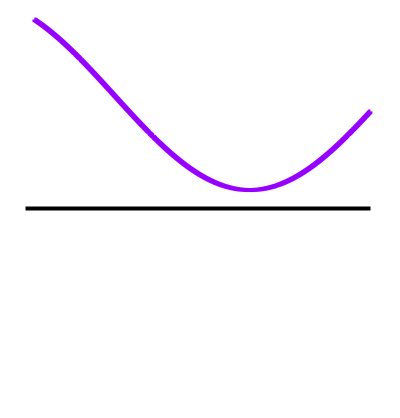
\includegraphics[height=3cm]{trichotomy-1}
  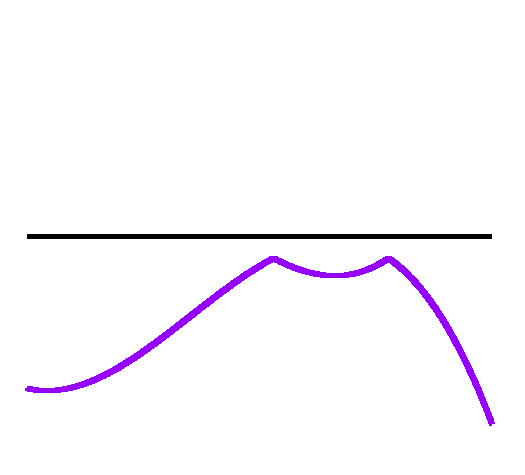
\includegraphics[height=3cm]{trichotomy-2}
  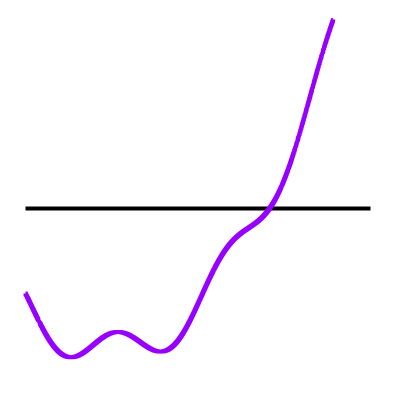
\includegraphics[height=3cm]{trichotomy-3}
  \caption{\label{fig:trichotomy} Three examples for what the topos~$\Sh(X)$
  each believes to be a single real number, where the base space~$X$ is the
  unit interval. (a) A positive real number. (b) A negative real number. (c) A
  number which is neither negative nor zero nor positive. Externally speaking,
  there is no covering of the unit interval by open subsets on which the
  depicted function~$a$ is either everywhere negative, everywhere zero or everywhere
  positive.}
\end{figure}


\subsection{Real functions} Let~$(f_x)_{x \in X}$ be a continuous family of
continuous real-valued functions; that is, each of the individual
functions~$f_x : \RR \to \RR$ should be continuous and moreover the map~$\RR
\times X \to \RR, (a,x) \mapsto f_x(a)$ should be continuous.
From the point of view of~$\Sh(X)$, this family looks like a single continuous
function~$f : \RR \to \RR$.

The internal statement that~$f(-1) < 0$ means that~$f_x(-1) < 0$ for all~$x \in
X$, and similarly so for being positive. More generally, if~$a$ and~$b$ are
continuous functions~$X \to \RR$ (hence real numbers from the internal point of
view), the internal statement~$f(a) < b$ means that~$f_x(a(x)) < b(x)$ for
all~$x \in X$.

The internal statement that~$f$ possesses a zero, that is, that there exists a
number~$a$ such that~$f(a) = 0$, means that all the functions~$f_x$ each
possess a zero and that moreover, these zeros can locally be picked in a
continuous fashion. More precisely, this statement means that there is an open
covering~$X = \bigcup_i U_i$ such that, for each~$i$, there is a continuous
function~$a : U_i \to \RR$ such that~$f_x(a(x)) = 0$ for all~$x \in U_i$. (On
overlaps~$U_i \cap U_j$, the zero-picking functions~$a$ need not agree.)

From these observations we can deduce that the intermediate value theorem of
basic analysis does in general not hold in~$\Sh(X)$ and hence does not allow
for an intuitionistic proof. This theorem states: ``If~$f : \RR \to \RR$
is a continuous function such that~$f(-1) < 0$ and~$f(1) > 0$, there exists a
number~$a$ such that~$f(a) = 0$.'' The external meaning of this statement is
that in any continuous family~$(f_x)_x$ of continuous functions with~$f_x(-1) <
0$ and~$f_x(1) > 0$ for all~$x \in X$, it's locally possible to pick zeros of
the family in a continuous fashion. Figure~\ref{fig:ivt} shows a counterexample
to this claim.

\printbibliography

\end{document}


Outline:


Stuff that should be mentioned:

* Andrej's realizability in the real world
* Cauchy vs. Dedekind numbers (physical quantities, ...)
* Syntactical vs. semantical interpretation
* phone call analogy
* detailed explanation of the pretty picture; analogy with "inner models"
  of set theory
* quick overview of the several aspects of toposes (maybe at the end,
  as an outlook?)
* enrichment of platonism debate (find better term for this!)
* uncovering further relations between objects
* allowing a switch of perspective
* applications in mathematical practice
* int. logic as common denominator
* arbitrariness of the "standard axioms"
* models of ZF yield toposes (models of ETCS), including a quick discussion of
  equivalence
* what giving up classical logic actually amounts to in practice
* examples in Spec(A), "reifying all the individual localizations into a
  single coherent entity which can be reasoned about as if it were a single
  ring"
* importance of having an adapted language
* SDG (infinitesimals are well-studied in philosophy of mathematics)
* quick remark on the internal language being based on types instead of sets
* reference to Bohr topos approach
* Source https://plato.stanford.edu/entries/category-theory/ for relevant
  literatur
* the internal language as a generalized modal operator

* use the phrase "very rich and very deep" (or similarly) about set theory

Send to Georg.
Also Giuseppe Cammarata.
